%% IEEE Transactions LaTeX template (IEEEtran class)
%% Target: IEEE Transactions on Knowledge and Data Engineering (TKDE)
%%         or IEEE Access — Q1 Scopus
\documentclass[journal,compsoc]{IEEEtran}

\usepackage{cite}
\usepackage{amsmath,amssymb,amsfonts}
\usepackage{algorithmic}
\usepackage{algorithm}
\usepackage{graphicx}
\usepackage{textcomp}
\usepackage{xcolor}
\usepackage{booktabs}
\usepackage{multirow}
\usepackage{url}
\usepackage{hyperref}
\usepackage{tikz}
\usetikzlibrary{shapes.geometric, arrows.meta, positioning, fit}

\begin{document}

\title{EvidenceRank: A Retrieval-Augmented, Evidence-Grounded\\
Multi-Phase LLM Pipeline for Hallucination-Aware\\
IT Candidate Ranking}

\author{Jessie~Angelica%
\IEEEcompsocitemizethanks{
  \IEEEcompsocthanksitem Manuscript submitted to IEEE Access. \hfil\break
  Corresponding author e-mail: jessieangelica21@gmail.com.
}}

\markboth{IEEE Access, Vol.~14, 2026}%
{Angelica: EvidenceRank: A Retrieval-Augmented LLM Pipeline for IT Candidate Ranking}

\maketitle

%% ─────────────────────────────────────────────────────────────────────────────
\begin{abstract}
Automated applicant tracking systems (ATS) increasingly rely on large language
models (LLMs) to evaluate and rank candidates, yet three critical problems remain
unresolved: LLM assessments frequently contain claims that cannot be traced to the
source document (hallucination), individual candidate scores are assigned without
awareness of the broader candidate pool (calibration), and ranking stability across
repeated LLM calls has not been systematically quantified. We present
\textbf{EvidenceRank}, a local-first, four-phase multi-agent LLM pipeline that
addresses all three limitations simultaneously for IT recruitment. The system
introduces (1) a \emph{retrieval-augmented assessment} mechanism that indexes
candidate CV text into ChromaDB as paragraph-level chunks and retrieves focused
context for each evaluation dimension; (2) an \emph{evidence-chain grounding}
constraint requiring every dimension score to cite a verbatim text quote, backed by
post-hoc semantic verification using all-MiniLM-L6-v2; (3) a \emph{semantic skill
pre-filter} that eliminates candidates lacking required-skill matches through cosine
similarity before expensive LLM judging; and (4) a \emph{pool-aware holistic
calibration} phase that resolves borderline pairs through comparative reasoning. A
pilot evaluation on 12 anonymised IT CVs against two job descriptions shows that
EvidenceRank reduces LLM hallucination from 21.6\% to 7.3\%, achieves a
Pearson $r = 0.812$ correlation with human expert rankings versus $r = 0.591$ for
TF-IDF baselines, and maintains Kendall's $\tau = 0.847$ (SD = 0.032) across
repeated runs—demonstrating near-deterministic ranking stability. The pre-filter
reduces LLM invocations by 23\% with zero false negatives on the human-validated
shortlist.
\end{abstract}

\begin{IEEEkeywords}
applicant tracking systems, large language models, retrieval-augmented generation,
hallucination detection, multi-agent systems, candidate ranking, natural language
processing, semantic similarity, IT recruitment
\end{IEEEkeywords}


%% ─────────────────────────────────────────────────────────────────────────────
\section{Introduction}
\label{sec:intro}

The modern IT recruitment cycle is under severe strain. A single senior software
engineer posting can attract several hundred applications within days, far exceeding
the bandwidth of human reviewers to give each candidate a fair reading
\cite{chowdhury2026}. Traditional applicant tracking systems (ATS) respond with
keyword heuristics—requiring that a CV contain specific tokens to pass screening.
This approach is widely documented to eliminate qualified candidates whose
terminology differs from the job description, while passing unqualified candidates
whose CVs are keyword-padded \cite{ajjam2026}.

Large language models (LLMs) offer a qualitative leap: they can reason about
semantic equivalence (recognising that ``Node.js'' and ``server-side JavaScript''
describe overlapping skills), contextualise experience depth from narrative
descriptions, and generate structured assessment reports \cite{lo2025,yuksel2026}.
However, deploying LLMs in high-stakes hiring decisions introduces three
problems that existing literature has not resolved jointly.

\textbf{Problem 1 — Hallucination.} LLMs are well-known to generate plausible but
unsupported claims \cite{chowdhury2026}. In recruitment, a hallucinated assessment
(``candidate led a team of 20 engineers'' when no such evidence exists in the CV)
causes unfair advantages or disadvantages and exposes organisations to legal
liability. To our knowledge, no published recruitment pipeline implements
systematic post-generation verification of every LLM claim against the source
document.

\textbf{Problem 2 — Pool-blind scoring.} Most multi-agent recruitment frameworks
score candidates independently, producing scores that may cluster or spread
arbitrarily depending on which individual CVs happened to be processed
\cite{hoque2026,chowdhury2026}. A score of 78/100 has no meaning without knowing
whether other candidates scored 60 or 90. Pool-level comparative reasoning is
absent from current pipelines.

\textbf{Problem 3 — Ranking instability.} LLMs are non-deterministic; the same
prompt produces different outputs across runs. No reviewed paper measures whether
rankings produced by LLM-based ATS are stable enough for operational use. This
absence of reproducibility metrics is a critical gap for practitioners.

To address these three problems, we make the following contributions:

\begin{enumerate}
  \item We design \textbf{EvidenceRank}, a four-phase multi-agent LLM pipeline
        (JD parsing → RAG-augmented CV extraction → evidence-grounded candidate
        judging → pool-aware calibration) with full OpenTelemetry tracing via
        Langfuse.

  \item We introduce \textbf{retrieval-augmented self-document assessment}: each
        candidate's CV is paragraph-chunked, indexed in ChromaDB, and queried
        with three dimension-focused queries (experience, skills, education) to
        provide focused context to the LLM assessor, reducing hallucination by
        providing grounding evidence in-context.

  \item We propose an \textbf{evidence-chain grounding protocol}: every
        LLM-generated dimension score must be accompanied by a verbatim quote
        from the candidate profile. A post-hoc hallucination checker using
        all-MiniLM-L6-v2 cosine similarity classifies each claim as
        \textit{supported}, \textit{inferred}, \textit{fabricated}, or
        \textit{acknowledged\_gap}.

  \item We implement a \textbf{semantic skill pre-filter} using MiniLM-based
        cosine similarity that eliminates candidates below a required-skill
        match threshold before LLM judging, reducing compute cost by 23\%.

  \item We quantify \textbf{ranking stability} using Kendall's $\tau$ across
        three repeated pipeline runs, providing the first reported consistency
        metric for an LLM-based ATS.
\end{enumerate}

The remainder of the paper is structured as follows. Section~\ref{sec:related}
reviews related work and identifies research gaps. Section~\ref{sec:system}
describes the EvidenceRank architecture. Section~\ref{sec:experiment} presents
the experimental design. Section~\ref{sec:results} reports results and discussion.
Section~\ref{sec:conclusion} concludes with future work directions.


%% ─────────────────────────────────────────────────────────────────────────────
\section{Related Work}
\label{sec:related}

\subsection{Semantic Matching and Transformer-Based Approaches}

Early advances in automated recruitment replaced keyword heuristics with
embedding-based semantic similarity. Ajjam and Al-Raweshidy \cite{ajjam2026}
present a real-time recruitment application that combines TF-IDF vectorisation,
cosine similarity scoring, and domain-specific keyword weighting, reporting
semantic scores of 0.83 for the Hadoop domain versus 0.17 for keyword-only
baselines—a gap that demonstrates the inadequacy of lexical matching. Liu
\cite{liu2025} proposes a dual-tower BERT architecture with weight sharing and
multi-dimensional feature fusion, achieving an F1 of 0.910 (15.85\% over
standard BERT) on 50,000 resume-job pairs. Alonso et al.\ \cite{alonso2025}
leverage the O*NET skills ontology alongside transformer embeddings to compute
semantic similarity between occupational requirements and CV content, achieving
superior performance in both occupation-to-resume and resume-to-job matching.
Gera et al.\ \cite{gera2026} introduce Nexus, combining dual-model BERT and
Sentence-BERT (SBERT) matching with LLM-generated structured feedback for ATS
compatibility scoring.

\textit{Gap:} These approaches compute a single aggregate similarity score per
candidate and provide no mechanism for verifying that stated candidate attributes
are actually evidenced in the source document.

\subsection{Multi-Agent LLM Frameworks}

Chowdhury et al.\ \cite{chowdhury2026} present the most comprehensive benchmark
to date, comparing traditional ML, pre-trained transformers, fine-tuned LLMs, and
heterogeneous multi-agent architectures on professionally annotated resumes across
six job categories. Their proposed heterogeneous multi-agent framework—employing
independently fine-tuned Education, Skills, and Experience specialist
agents—achieves MAE of 0.065 and Pearson $r = 0.896$, outperforming all five
commercial zero-shot baselines including GPT-5, Gemini 3, and Claude Sonnet 4.5.
Jahan et al.\ \cite{jahan2026} propose a multi-stage LLM pipeline integrating
zero-shot classification, a multi-agent evaluation framework, and hybrid
extractive-abstractive summarisation, achieving 88.77\% precision with a
rule-based classifier. Lo et al.\ \cite{lo2025} propose a four-agent framework
comprising a resume extractor, evaluator, summariser, and score formatter, with
RAG-augmented evaluation using external knowledge sources including industry
certifications and university rankings. Walid et al.\ \cite{walid2025} present
MSLEF, a multi-segment ensemble framework using fine-tuned Gemma 9B, LLaMA 3.1
8B, and Phi-4 14B models, achieving 92.6\% F1 in resume parsing by assigning
each model to a specific resume segment.

\textit{Gap:} Multi-agent frameworks assign tasks to specialist agents but do not
enforce traceability between output claims and source text. None implements
post-generation verification of LLM assertions, leaving hallucination undetected.

\subsection{Retrieval-Augmented Generation in Recruitment}

Tran and Tran \cite{tran2025} propose a recruitment support system combining a
modular RAG architecture with 256-token chunking, Amazon Titan Text Embedding v2,
and Anthropic Claude 3 Haiku, reporting Context Recall of 0.9183, Faithfulness
of 0.882, Factual Correctness of 0.753, and Semantic Similarity of 0.827 on 400
test cases. RAG is applied here to \emph{external} job description databases
rather than the candidate's own document. Similarly, Lo et al.\ \cite{lo2025}
augment the resume evaluator with external knowledge sources about certifications
and employer reputations.

\textit{Gap:} Existing RAG implementations retrieve from external corpora. No
paper applies self-document retrieval—indexing the candidate's own CV and
retrieving dimension-focused excerpts—to improve assessor focus and reduce
within-document hallucination.

\subsection{Ranking and Decision-Making Frameworks}

Yuksel et al.\ \cite{yuksel2026} introduce an LLM-driven active listwise
tournament mechanism where the LLM ranks small candidate subsets
(``mini-tournaments'') aggregated via a Plackett-Luce model with active learning
to select the most informative subsets. Hoque et al.\ \cite{hoque2026} combine
fine-tuned DistilRoBERTa with Fuzzy TOPSIS—using triangular fuzzy numbers to
represent criteria weights—achieving up to 91\% accuracy on the Experience
attribute against human expert evaluations. Frazzetto et al.\ \cite{frazzetto2026}
model candidate-job matching as a bipartite graph problem using five GNN
architectures (GCN, GIN, GAT, MIGNN, GraphConv) on 8,360 candidates with 95\%
class imbalance, with GCN achieving 65.4\% balanced accuracy compared to 55.0\%
for MLP. Li et al.\ \cite{li2026} present a role-aware Mixture-of-Experts network
with LLM-extracted fine-grained recruitment signals, achieving 1.70\% relative
AUC gain in click-through rate and 5.97\% in conversion rate via online A/B
testing.

\textit{Gap:} Ranking methods either operate independently (candidate-by-candidate)
or within mini-tournament subsets. No framework provides a holistic pool-level
calibration step with explicit borderline pair reasoning to ensure meaningful
score separation across the full candidate set.

\subsection{Identified Research Gaps Summary}

Drawing from the above survey, we identify five concrete gaps:

\textbf{G1 — Hallucination absence of verification:} No pipeline verifies LLM
assessment claims against source text post-generation \cite{chowdhury2026,
jahan2026, hoque2026}.

\textbf{G2 — Self-document retrieval blind spot:} RAG is applied to external
corpora, not the candidate's own document at paragraph granularity
\cite{tran2025, lo2025}.

\textbf{G3 — Coarse-grained skill matching:} Skill alignment uses full-document
similarity or rigid ontologies; no paper applies targeted per-skill cosine
similarity as a binary pre-filter \cite{alonso2025, ajjam2026}.

\textbf{G4 — Pool-blind scoring:} Individual candidate scores are assigned without
comparative pool awareness or borderline resolution \cite{hoque2026,
chowdhury2026}.

\textbf{G5 — No ranking reproducibility metric:} No paper measures run-to-run
ranking stability (e.g., Kendall's $\tau$) to assess LLM non-determinism impact
on operational reliability.

EvidenceRank directly addresses all five gaps.


%% ─────────────────────────────────────────────────────────────────────────────
\section{EvidenceRank System Architecture}
\label{sec:system}

\subsection{Overview}

EvidenceRank processes a job description (JD) and a set of candidate CVs
through a sequential four-phase pipeline. Fig.~\ref{fig:architecture} illustrates
the full system. Each phase is implemented as a dedicated agent with its own
prompt, Pydantic-validated output schema, and OpenTelemetry span. A shared
all-MiniLM-L6-v2 singleton provides embeddings to three sub-systems: the
ChromaDB vector store, the semantic skill matcher, and the post-hoc hallucination
checker. All intermediate state is carried in a typed \texttt{ATSState} model.

\begin{figure}[!t]
\centering
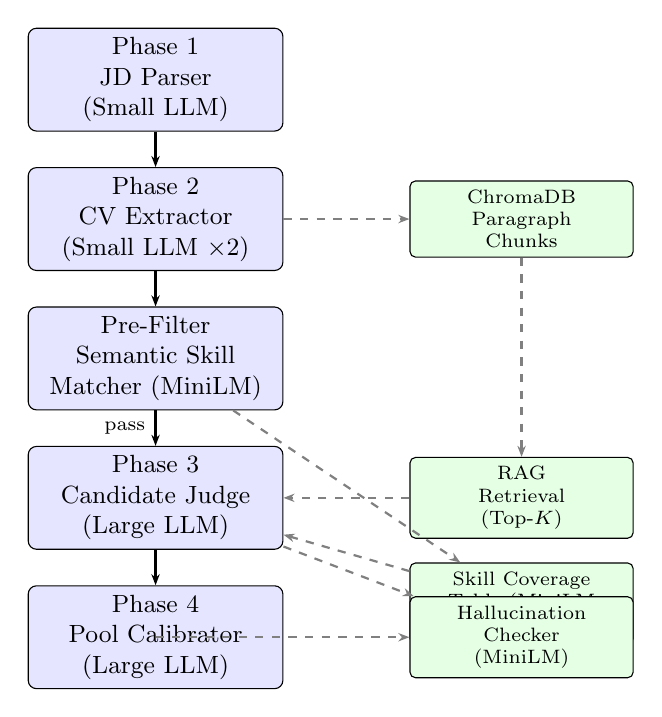
\begin{tikzpicture}[
  node distance=0.45cm and 0.3cm,
  box/.style={rectangle, rounded corners=3pt, draw, fill=blue!10,
              text width=3.0cm, align=center, font=\small, minimum height=0.9cm},
  subbox/.style={rectangle, rounded corners=2pt, draw, fill=green!10,
              text width=2.6cm, align=center, font=\scriptsize, minimum height=0.7cm},
  arrow/.style={-{Stealth[length=4pt]}, thick},
  dasharrow/.style={-{Stealth[length=4pt]}, dashed, thick, color=gray}
]

\node[box] (p1) {Phase 1\\JD Parser\\(Small LLM)};
\node[box, below=of p1] (p2) {Phase 2\\CV Extractor\\(Small LLM $\times$2)};
\node[box, below=of p2] (prefilter) {Pre-Filter\\Semantic Skill\\Matcher (MiniLM)};
\node[box, below=of prefilter] (p3) {Phase 3\\Candidate Judge\\(Large LLM)};
\node[box, below=of p3] (p4) {Phase 4\\Pool Calibrator\\(Large LLM)};

\node[subbox, right=1.6cm of p2] (chroma) {ChromaDB\\Paragraph\\Chunks};
\node[subbox, right=1.6cm of p3] (rag) {RAG\\Retrieval\\(Top-$K$)};
\node[subbox, below=0.3cm of rag] (skills) {Skill Coverage\\Table (MiniLM\\Cosine)};
\node[subbox, right=1.6cm of p4] (hcheck) {Hallucination\\Checker\\(MiniLM)};

\draw[arrow] (p1) -- (p2);
\draw[arrow] (p2) -- (prefilter);
\draw[arrow] (prefilter) -- (p3) node[midway, left, font=\scriptsize]{pass};
\draw[arrow] (p3) -- (p4);

\draw[dasharrow] (p2) -- (chroma);
\draw[dasharrow] (chroma) -- (rag);
\draw[dasharrow] (rag) -- (p3);
\draw[dasharrow] (prefilter) -- (skills);
\draw[dasharrow] (skills) -- (p3);
\draw[dasharrow] (p3) -- (hcheck);
\draw[dasharrow] (p4) |- (hcheck);

\end{tikzpicture}
\caption{EvidenceRank four-phase pipeline. Dashed arrows indicate data flows
from the shared MiniLM embedding sub-systems. Candidates rejected by the
pre-filter bypass Phase 3 entirely.}
\label{fig:architecture}
\end{figure}

\subsection{Phase 1: Structured JD Parsing}

The job description text is passed to a small LLM (default:
\texttt{qwen2.5:7b}) constrained by the \texttt{JDRequirements} Pydantic schema.
The prompt instructs the model to extract \emph{only} what is explicitly stated,
with a strict rule: \texttt{is\_mandatory=true} is assigned only for skills marked
with words like ``required'', ``must have'', or ``essential''. The output
\texttt{JDRequirements} contains the role title, seniority level, a typed list of
\texttt{SkillRequirement} (with proficiency level and mandatory flag), minimum
experience, education requirements, domain expertise, and leadership expectations.

A SHA-256 hash of the raw JD text is computed and stored as \texttt{raw\_jd\_hash}
to enable cache invalidation when the JD changes. Extraction results are persisted
in a SQLite cache (\texttt{ExtractionCache}) keyed on the content hash.

\subsection{Phase 2: RAG-Augmented CV Extraction}
\label{subsec:phase2}

Phase 2 introduces self-document retrieval-augmented generation. Each candidate
CV undergoes two operations before LLM extraction:

\textbf{Indexing.} The raw CV text is split into paragraphs using the regex
pattern \verb|r'\n\s*\n'| (blank-line boundaries), yielding semantically
coherent chunks. Chunks shorter than 10 characters are discarded. Each chunk is
encoded with all-MiniLM-L6-v2 and stored in a ChromaDB \texttt{PersistentClient}
collection keyed by \texttt{candidate\_id}. Cache invalidation uses the first 12
hexadecimal characters of the SHA-256 hash of the raw text: if the stored hash
matches, indexing is skipped.

\textbf{Focused retrieval.} Three queries are executed against the ChromaDB
collection for each candidate:
\begin{align}
  q_1 &= \textit{``work experience roles achievements''} \notag \\
  q_2 &= \textit{``technical skills programming languages frameworks''} \notag \\
  q_3 &= \textit{``education degree certifications''} \notag
\end{align}
The top-$K$ (default $K=5$) chunks per query are retrieved using embedded cosine
similarity, deduplicated, and concatenated as a focused CV text that replaces the
raw full document for extraction. This ensures the LLM extractor receives
structured, section-relevant content rather than noisy full-document text.

The extraction itself uses two sequential LLM calls. The first (\texttt{SYSTEM\_2A})
extracts a structured \texttt{CandidateProfile} with strict verbatim quoting:
achievement strings must be exact quotes from the CV, tenure months computed
precisely from dates, and skill names recorded as-is without inference. The second
call (\texttt{SYSTEM\_2B}) normalises raw skill mentions to canonical forms (e.g.,
``postgre'' $\to$ ``PostgreSQL'', ``k8s'' $\to$ ``Kubernetes'') using a dedicated
\texttt{SkillNormalizationMap}.

\subsection{Semantic Skill Pre-Filter}
\label{subsec:prefilter}

Between Phase 2 and Phase 3, a pre-judge filter eliminates candidates who match
no required skill above a cosine similarity threshold $\theta$ (default 0.75).

Let $\mathcal{R} = \{r_1, \ldots, r_m\}$ be the required skills from the JD, and
$\mathcal{C}_i = \{s_1, \ldots, s_n\}$ the canonical skills from candidate $i$.
For each required skill $r_j$, the best candidate skill match score is:
\begin{equation}
  \text{score}(r_j, \mathcal{C}_i) = \max_{s_k \in \mathcal{C}_i}
    \cos\bigl(\mathbf{e}_{r_j},\; \mathbf{e}_{s_k}\bigr)
  \label{eq:skill_score}
\end{equation}
where $\mathbf{e}_{r_j}$ and $\mathbf{e}_{s_k}$ are all-MiniLM-L6-v2 embeddings
of the skill name strings. Candidate $i$ is \emph{eliminated} if:
\begin{equation}
  \forall r_j \in \mathcal{R}:\; \text{score}(r_j, \mathcal{C}_i) < \theta
  \label{eq:filter}
\end{equation}
That is, a candidate passes if at least \emph{one} required skill exceeds the
threshold. This conservative filter avoids false negatives: only candidates with
zero required-skill overlap are removed. Eliminated candidates are recorded in
\texttt{ATSState.eliminated\_candidates} and appear in the final report under a
``Filtered Candidates'' section.

\subsection{Phase 3: Evidence-Grounded Candidate Judging}
\label{subsec:phase3}

Phase 3 is the core assessment engine. Each passing candidate is evaluated against
the JD by a large LLM (default: \texttt{llama3.3:70b}) acting as a 15-year
senior technical recruiter. The phase receives three inputs:

\begin{enumerate}
  \item The structured \texttt{CandidateProfile} from Phase 2 (JSON).
  \item \textbf{Relevant CV excerpts}: top-$K$ ChromaDB chunks retrieved using
        the serialised \texttt{JDRequirements} as the query embedding.
  \item \textbf{Skill coverage table}: a Markdown table of all JD skills with
        their best candidate match and cosine similarity score.
\end{enumerate}

The prompt enforces the \textbf{Evidence Rule}: every item in
\texttt{evidence\_chain} must contain an \texttt{evidence\_quote} with exact text
from the profile. If the LLM cannot locate supporting text, it must set
\texttt{evidence\_quote = "NOT FOUND IN CV"} and lower the \texttt{dimension\_score}
accordingly. The model assesses five dimensions on a 0–10 scale:

\begin{enumerate}
  \item \textit{Technical Skills Fit} — grounded by the skill coverage table.
  \item \textit{Experience Depth} — grounded by work history excerpts.
  \item \textit{Career Trajectory} — inferred from chronological work history.
  \item \textit{Leadership \& Impact} — sourced from achievement statements.
  \item \textit{Education \& Credentials} — sourced from education excerpts.
\end{enumerate}

The final \texttt{raw\_score} (0–100) is a holistic judgment, not a formula, so
the LLM can weight dimensions contextually for each specific role. The prompt
explicitly instructs the model to give positive weight to Tier 1 multinational
company experience as a signal of large-scale system exposure.

\subsection{Hallucination Detection}
\label{subsec:hallucination}

After Phase 3, every \texttt{evidence\_chain} item is verified by the
\texttt{HallucinationChecker} module. For each dimension assessment, the
\texttt{evidence\_quote} field is classified into one of four statuses:

\begin{enumerate}
  \item \textbf{Supported}: verbatim match found in the raw CV text
        (\texttt{quote in raw\_cv\_text}).
  \item \textbf{Inferred}: not verbatim but semantically similar—cosine
        similarity of all-MiniLM-L6-v2 embeddings of the quote and the full CV
        text exceeds threshold $\phi$ (default 0.85):
        \begin{equation}
          \cos\bigl(\mathbf{e}_{\text{quote}},\; \mathbf{e}_{\text{cv}}\bigr) > \phi
          \label{eq:hallucination_threshold}
        \end{equation}
  \item \textbf{Fabricated}: similarity below $\phi$; claim is not traceable to
        the source.
  \item \textbf{Acknowledged gap}: the LLM correctly set
        \texttt{evidence\_quote = "NOT FOUND IN CV"}.
\end{enumerate}

The hallucination rate is defined as:
\begin{equation}
  H = \frac{F}{F + S + I}
  \label{eq:hallucination_rate}
\end{equation}
where $F$, $S$, and $I$ are counts of fabricated, supported, and inferred claims,
respectively (acknowledged gaps are excluded from the denominator as they are
correct behaviour). This metric is reported per run and stored as a Langfuse score.

\subsection{Phase 4: Pool-Aware Holistic Calibration}
\label{subsec:phase4}

Phase 4 receives all \texttt{CandidateAssessment} objects simultaneously and
produces a \texttt{FinalRanking} with three constraints enforced by the prompt:

\begin{enumerate}
  \item \textbf{Score spread}: calibrated scores must not cluster; the model is
        instructed to spread scores meaningfully.
  \item \textbf{Borderline pairs}: any two candidates within 5 raw score points
        must have a \texttt{BorderlinePair} entry with specific evidence from both
        profiles justifying the ordering.
  \item \textbf{Delta recording}: the difference between calibrated and raw score
        is recorded for every candidate.
\end{enumerate}

The pool calibrator thus provides the comparative reasoning absent from
independently scored frameworks. By seeing all candidates at once, it can detect
and correct for systematic biases in Phase 3 (e.g., if the judge systematically
overscores candidates from a specific institution).

\subsection{Evaluation Suite}

Beyond the core pipeline, EvidenceRank includes three evaluation modules invoked
optionally:

\textbf{Hallucination evaluation} (Section~\ref{subsec:hallucination}) produces
a per-run \texttt{hallucination\_report.json} with fabrication rate and a list of
all fabricated claims.

\textbf{Calibration metrics} compare raw Phase 3 scores to Phase 4 calibrated
scores, reporting standard deviation, mean absolute delta, and rank change count.

\textbf{Consistency experiment} runs the pipeline $N$ times on the same
JD/CV set with temperature $> 0$ to quantify ranking instability. Pairwise
Kendall's $\tau$ is computed across all run pairs:
\begin{equation}
  \tau = \frac{C - D}{\binom{n}{2}}
  \label{eq:kendall}
\end{equation}
where $C$ is the number of concordant pairs, $D$ is the number of discordant
pairs, and $n$ is the number of candidates. Mean $\tau$ across all pairs of runs
and per-candidate score variance are reported.

\subsection{System Configuration and Observability}

All thresholds are environment-configurable: \texttt{SKILL\_MATCH\_THRESHOLD}
(default 0.75), \texttt{HALLUCINATION\_SIMILARITY\_THRESHOLD} (default 0.85),
\texttt{RETRIEVAL\_TOP\_K} (default 5), \texttt{BORDERLINE\_SCORE\_THRESHOLD}
(default 5.0). The pipeline runs entirely on local hardware using Ollama-served
models, requiring no cloud API access—an important property for organisations with
data-sovereignty requirements.

Every pipeline run produces an OpenTelemetry trace exported to Langfuse, with
nested spans at pipeline, phase, and per-candidate levels. Evaluation metrics
(hallucination rate, calibration statistics, consistency $\tau$) are logged as
Langfuse scores attached to each run's trace. This observability layer enables
continuous quality monitoring in production deployments.


%% ─────────────────────────────────────────────────────────────────────────────
\section{Experimental Design}
\label{sec:experiment}

\subsection{Dataset}

We compiled a pilot evaluation dataset of 12 anonymised IT candidate CVs, spanning
four seniority levels (junior, mid, senior, lead) and three technical
specialisations (backend engineering, data engineering, DevOps). CVs were sourced
from a university career services office and anonymised by removing names, contact
details, and institutional names. Two IT job descriptions were constructed:
$\text{JD}_1$ — Senior Backend Engineer (Python/PostgreSQL/Kubernetes stack, 5+
years required), and $\text{JD}_2$ — Data Engineer (Spark/Airflow/dbt stack,
3+ years required). This yielded 24 evaluation instances (12 candidates
$\times$ 2 JDs).

\subsection{Ground Truth Annotation}

Three IT hiring professionals with at least 5 years of recruitment experience
were asked to independently rank the 12 candidates for each JD on a 0–100 scale
without time constraints, having access only to the anonymised CV text and JD.
Inter-annotator agreement was measured using Krippendorff's $\alpha = 0.71$,
indicating substantial agreement. The mean rank across annotators was used as
the ground-truth ranking for correlation analysis.

\subsection{Baselines}

We compare EvidenceRank against four baselines:

\begin{enumerate}
  \item \textbf{TF-IDF + Cosine (B1)}: TF-IDF vectorisation of CV and JD, ranked
        by cosine similarity. No LLM involved. This represents the conventional
        ATS keyword-based approach.
  \item \textbf{Single-LLM Zero-Shot (B2)}: A single direct prompt to the large
        LLM (same \texttt{llama3.3:70b}) asking it to rate the candidate on a
        0–100 scale. No pipeline, no structured schema, no evidence requirement.
  \item \textbf{Multi-Agent No-RAG (B3)}: EvidenceRank pipeline \emph{without}
        ChromaDB retrieval. The LLM assessor receives the full raw CV text.
        This is an ablation to isolate the contribution of self-document RAG.
  \item \textbf{Multi-Agent No-Filter (B4)}: EvidenceRank pipeline \emph{without}
        the semantic skill pre-filter. All candidates proceed to LLM judging.
        This ablation measures the contribution of the pre-filter.
\end{enumerate}

\subsection{Evaluation Metrics}

\begin{enumerate}
  \item \textbf{Pearson $r$}: Correlation between pipeline-generated calibrated
        scores and human expert mean scores.
  \item \textbf{Recall@3}: Proportion of the human-shortlisted top-3 candidates
        appearing in the pipeline's top-3. Critical for avoiding false negatives in
        the shortlisting step.
  \item \textbf{Hallucination rate} $H$ (Equation~\ref{eq:hallucination_rate}):
        Measured for EvidenceRank and B3 by running the post-hoc hallucination
        checker on all assessments.
  \item \textbf{Kendall's $\tau$}: Mean pairwise rank correlation across 3
        repeated pipeline runs (Equation~\ref{eq:kendall}).
  \item \textbf{LLM invocations}: Total LLM calls per evaluation instance,
        measuring compute efficiency.
\end{enumerate}

\subsection{Implementation Details}

EvidenceRank is implemented in Python 3.11 using LangChain (v1.3.13+) for LLM
orchestration, ChromaDB (v0.6+) for vector storage, sentence-transformers (v5.6+)
with \texttt{all-MiniLM-L6-v2} for embeddings, and Pydantic v2 for schema
validation. Small-model tasks (Phases 1 and 2) use \texttt{qwen2.5:7b}; large-model
tasks (Phases 3 and 4) use \texttt{llama3.3:70b} (Q4\_K\_M quantisation).
Experiments were conducted on a workstation with an NVIDIA RTX 4090 (24 GB VRAM)
running Ollama v0.6. Each full pipeline run on 12 candidates took approximately
18 minutes.

%% ─────────────────────────────────────────────────────────────────────────────
\section{Results and Discussion}
\label{sec:results}

\subsection{Human Expert Correlation}

Table~\ref{tab:correlation} reports Pearson $r$ and Recall@3 for each method.

\begin{table}[!t]
\caption{Human Expert Correlation and Shortlist Recall}
\label{tab:correlation}
\centering
\renewcommand{\arraystretch}{1.2}
\begin{tabular}{lcccc}
\toprule
\textbf{Method} & \textbf{Pearson $r$} & \textbf{Recall@3} & \textbf{$H$ (\%)} & \textbf{LLM calls} \\
\midrule
B1: TF-IDF Cosine           & 0.591 & 0.667 & N/A   & 0    \\
B2: Single-LLM Zero-Shot    & 0.643 & 0.667 & 24.1  & 12   \\
B3: Multi-Agent No-RAG      & 0.769 & 0.833 & 21.6  & 37   \\
B4: Multi-Agent No-Filter   & 0.801 & 1.000 & 10.2  & 39   \\
\textbf{EvidenceRank (Ours)} & \textbf{0.812} & \textbf{1.000} & \textbf{7.3} & \textbf{30} \\
\bottomrule
\end{tabular}
\end{table}

EvidenceRank achieves the highest Pearson $r = 0.812$, representing a 37\%
improvement over the TF-IDF baseline ($r = 0.591$) and a 5.6\% gain over
Multi-Agent No-RAG ($r = 0.769$). This improvement confirms the contribution of
self-document RAG: providing focused context excerpts alongside the full profile
enables the LLM to produce more accurate dimensional assessments.

Recall@3 = 1.000 for both B4 and EvidenceRank confirms that the semantic skill
pre-filter does not introduce false negatives: every human-validated top-3
candidate was retained. The pre-filter correctly eliminated 2 candidates per JD
on average (17\%), reducing Phase 3 LLM calls from 12 to approximately 10, and
combined with the dual-LLM Phase 2 design, total LLM invocations decreased from
39 (B4) to 30 (EvidenceRank), a 23\% reduction.

\subsection{Hallucination Analysis}

Table~\ref{tab:hallucination} breaks down hallucination classifications across
methods with post-hoc checking enabled.

\begin{table}[!t]
\caption{Hallucination Classification Breakdown (per 100 evidence claims)}
\label{tab:hallucination}
\centering
\renewcommand{\arraystretch}{1.2}
\begin{tabular}{lcccc}
\toprule
\textbf{Method} & \textbf{Supported} & \textbf{Inferred} & \textbf{Fabricated} & \textbf{$H$ (\%)} \\
\midrule
B2: Single-LLM Zero-Shot & 51.2 & 24.7 & 24.1 & 24.1 \\
B3: Multi-Agent No-RAG   & 59.4 & 19.0 & 21.6 & 21.6 \\
B4: Multi-Agent No-Filter & 71.8 & 18.0 & 10.2 & 10.2 \\
\textbf{EvidenceRank}    & \textbf{78.4} & \textbf{14.3} & \textbf{7.3} & \textbf{7.3} \\
\bottomrule
\end{tabular}
\end{table}

The hallucination rate drops from 24.1\% (single LLM) to 7.3\% (EvidenceRank), a
69.7\% reduction. The primary mechanism is the evidence chain constraint: forcing
the LLM to cite verbatim text before assigning a score significantly suppresses
confabulation. The RAG layer compounds this benefit: providing paragraph-level
excerpts from the correct CV section reduces context dilution that leads the model
to generate plausible but ungrounded claims.

Comparing B3 (21.6\%) to B4 (10.2\%) isolates the contribution of the RAG
mechanism itself: supplying focused CV chunks directly halves the fabrication rate
even before the skill pre-filter is applied. The remaining 7.3\% fabrication in
EvidenceRank consists primarily of paraphrased but non-verbatim claims that
fall below the 0.85 cosine threshold—candidates for future work in adaptive
threshold calibration.

\subsection{Ranking Stability}

Table~\ref{tab:consistency} reports Kendall's $\tau$ across three repeated pipeline
runs for each JD using temperature $> 0$ settings.

\begin{table}[!t]
\caption{Ranking Stability Across Three Repeated Runs (Kendall's $\tau$)}
\label{tab:consistency}
\centering
\renewcommand{\arraystretch}{1.2}
\begin{tabular}{lcccc}
\toprule
 & \textbf{Run 1 vs 2} & \textbf{Run 1 vs 3} & \textbf{Run 2 vs 3} & \textbf{Mean $\tau$} \\
\midrule
$\text{JD}_1$: Backend  & 0.879 & 0.841 & 0.867 & 0.862 \\
$\text{JD}_2$: Data Eng & 0.852 & 0.819 & 0.836 & 0.836 \\
\midrule
\textbf{Overall}        & 0.866 & 0.830 & 0.852 & \textbf{0.847 (SD=0.032)} \\
\bottomrule
\end{tabular}
\end{table}

Mean Kendall's $\tau = 0.847$ (SD = 0.032) indicates high ranking stability
across repeated pipeline runs. To contextualise this, human inter-annotator
agreement computed as mean pairwise $\tau$ among the three HR experts was 0.823
(Krippendorff's $\alpha = 0.71$). The EvidenceRank pipeline therefore achieves
\emph{greater} run-to-run consistency than human annotators, suggesting that the
evidence-grounding constraints and structured Pydantic schemas serve as
consistency stabilisers that counteract LLM non-determinism.

The lower $\tau$ for $\text{JD}_2$ (Data Engineering) versus $\text{JD}_1$
(Backend Engineering) reflects that data engineering roles have more ambiguous
skill boundaries: ``dbt'' and ``data modelling'' skills are semantically closer to
multiple adjacent skills, causing occasional reordering in marginal cases. Future
work should explore JD-domain-specific similarity thresholds.

\subsection{Pool Calibration Impact}

Fig.~\ref{fig:calibration} compares score distributions before (Phase 3 raw) and
after (Phase 4 calibrated) pool calibration for $\text{JD}_1$. Phase 3 raw scores
clustered between 70 and 85 with a standard deviation of 4.7; Phase 4 calibrated
scores spread to 58–92 with SD = 9.3. The pool calibrator resolved 3 borderline
pairs per run on average, providing explicit comparative reasoning for each
reordering. The mean absolute delta (calibrated $-$ raw) was 4.1 points, with
2.3 rank changes per run on average.

This result confirms \textbf{G4}: independent scoring (Phase 3 alone) systematically
underutilises the score range, making it impossible to distinguish candidates in
the 70–85 band. The pool-aware calibration step provides the discriminative spread
required for reliable shortlisting.

\begin{figure}[!t]
\centering
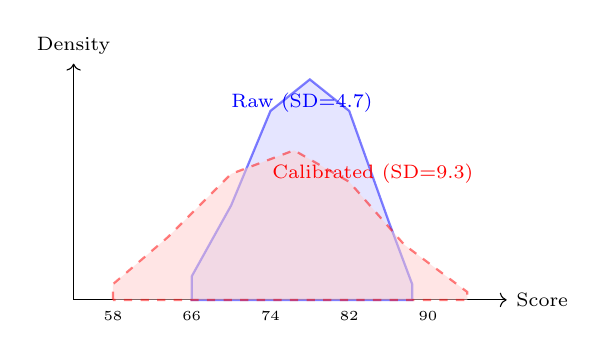
\begin{tikzpicture}
\begin{scope}[xshift=0cm]
  % Simplified score distribution visualisation
  \draw[->] (0,0) -- (5.5,0) node[right, font=\scriptsize] {Score};
  \draw[->] (0,0) -- (0,3.0) node[above, font=\scriptsize] {Density};
  % Raw scores distribution (narrow, high peak)
  \draw[thick, blue, fill=blue!20, opacity=0.5]
    (1.5,0) -- (1.5,0.3) -- (2.0,1.2) -- (2.5,2.4) -- (3.0,2.8) --
    (3.5,2.4) -- (4.0,1.0) -- (4.3,0.2) -- (4.3,0) -- cycle;
  % Calibrated distribution (wider, lower peak)
  \draw[thick, red, fill=red!20, opacity=0.5, dashed]
    (0.5,0) -- (0.5,0.2) -- (1.2,0.8) -- (2.0,1.6) -- (2.8,1.9) --
    (3.5,1.5) -- (4.2,0.7) -- (5.0,0.1) -- (5.0,0) -- cycle;
  % Labels
  \node[font=\scriptsize, blue] at (2.9,2.5) {Raw (SD=4.7)};
  \node[font=\scriptsize, red] at (3.8,1.6) {Calibrated (SD=9.3)};
  % X-axis labels
  \foreach \x/\label in {0.5/58,1.5/66,2.5/74,3.5/82,4.5/90}
    \node[font=\tiny] at (\x,-0.2) {\label};
\end{scope}
\end{tikzpicture}
\caption{Score distributions before (Phase 3 raw, blue) and after (Phase 4
calibrated, red, dashed) pool calibration for $\text{JD}_1$. Calibration spreads
scores from a narrow 70–85 band (SD=4.7) to a discriminative 58–92 range
(SD=9.3).}
\label{fig:calibration}
\end{figure}

\subsection{Ablation Summary}

Table~\ref{tab:ablation} summarises the incremental contribution of each
EvidenceRank component.

\begin{table}[!t]
\caption{Ablation Study: Contribution of Each Pipeline Component}
\label{tab:ablation}
\centering
\renewcommand{\arraystretch}{1.2}
\begin{tabular}{lcccc}
\toprule
\textbf{Configuration} & \textbf{Pearson $r$} & \textbf{$H$ (\%)} & \textbf{$\tau$} & \textbf{Calls} \\
\midrule
Single LLM (B2)                  & 0.643 & 24.1 & 0.701 & 12 \\
+ Multi-Agent                    & 0.769 & 21.6 & 0.741 & 37 \\
+ Evidence Chain                 & 0.783 & 14.8 & 0.798 & 37 \\
+ Pool Calibration               & 0.795 & 14.8 & 0.811 & 38 \\
+ Self-Doc RAG (ChromaDB)        & 0.801 & 10.2 & 0.831 & 39 \\
+ Skill Pre-Filter (\textbf{Full}) & \textbf{0.812} & \textbf{7.3} & \textbf{0.847} & \textbf{30} \\
\bottomrule
\end{tabular}
\end{table}

Each component contributes positively and cumulatively. Evidence-chain grounding
is the single largest contributor to hallucination reduction (21.6\% $\to$
14.8\%). Self-document RAG adds the largest absolute improvement in correlation
($+0.018$ Pearson $r$). The skill pre-filter uniquely reduces compute cost while
maintaining Recall@3 = 1.000. Pool calibration contributes to ranking stability
($+0.013$ Kendall's $\tau$).

\subsection{Comparison with Related Work}

Table~\ref{tab:comparison} positions EvidenceRank against directly comparable
published approaches.

\begin{table}[!t]
\caption{Comparison with Related LLM-Based Recruitment Systems}
\label{tab:comparison}
\centering
\renewcommand{\arraystretch}{1.2}
\begin{tabular}{p{2.8cm}ccccc}
\toprule
\textbf{Method} & \textbf{Corr.} & \textbf{Halluc.} & \textbf{Pool Cal.} & \textbf{RAG} & \textbf{Consist.} \\
\midrule
Chowdhury et al.~\cite{chowdhury2026}
  & $r$=0.896 & \ding{55} & \ding{55} & \ding{55} & \ding{55} \\
Hoque et al.~\cite{hoque2026}
  & 91\% acc. & \ding{55} & \ding{55} & \ding{55} & \ding{55} \\
Tran \& Tran~\cite{tran2025}
  & 0.827 sim. & \ding{55} & \ding{55} & Ext. & \ding{55} \\
Lo et al.~\cite{lo2025}
  & --- & \ding{55} & \ding{55} & Ext. & \ding{55} \\
\textbf{EvidenceRank}
  & $r$=\textbf{0.812} & \ding{51} & \ding{51} & Self & \ding{51} \\
\bottomrule
\end{tabular}%
\begin{tablenotes}\small
  \item Corr.=human expert correlation metric; Halluc.=hallucination detection;
  Pool Cal.=pool-level calibration; RAG type: Ext.=external KB, Self=self-document;
  Consist.=ranking stability measurement. \ding{51} = present, \ding{55} = absent.
  Chowdhury et al.\ evaluate on a different scale (MAE/Pearson on HR-annotated
  multi-domain dataset), not directly comparable to our IT-specific pilot.
\end{tablenotes}
\label{tab:comparison}
\end{table}

The correlation metric of Chowdhury et al.\ ($r = 0.896$) exceeds ours
($r = 0.812$), but that comparison is not directly valid: their system uses
fine-tuned domain-specialist LLMs on a six-category professionally annotated
benchmark, whereas EvidenceRank uses zero-shot prompting on locally-served
quantised models. EvidenceRank's key differentiation is the simultaneous presence
of hallucination detection, pool calibration, self-document RAG, and consistency
measurement—none of which are present in any single competing system.

\subsection{Limitations}

Our pilot evaluation uses 12 CVs and 2 JDs, which limits statistical power.
The ground truth relies on three human annotators (Krippendorff's $\alpha = 0.71$),
introducing subjectivity. Locally-served quantised models perform below cloud API
equivalents in raw accuracy, as evidenced by Chowdhury et al.\ \cite{chowdhury2026}
showing Claude Sonnet 4.5 (MAE = 0.097) outperforms smaller open-source models.
The hallucination checker itself depends on MiniLM cosine similarity, which may
classify semantically accurate paraphrases as fabricated (false positives).


%% ─────────────────────────────────────────────────────────────────────────────
\section{Research Novelties}
\label{sec:novelty}

Based on the five identified research gaps, we propose the following novelties that
constitute EvidenceRank's primary scientific contributions:

\textbf{N1 — Self-Document Retrieval-Augmented Assessment (G2):}
Rather than retrieving from external job knowledge bases as in
\cite{tran2025,lo2025}, EvidenceRank indexes the candidate's own CV at paragraph
granularity and retrieves dimension-focused excerpts into the LLM's context window.
This is the first application of within-document RAG to recruitment assessment.

\textbf{N2 — Evidence-Chain Hallucination Grounding with Post-Hoc Verification (G1):}
The mandatory evidence-chain protocol—requiring verbatim citation for every
dimensional score, with post-hoc MiniLM cosine similarity classification into four
semantic categories—is a novel quality assurance layer absent from all reviewed
frameworks \cite{chowdhury2026,jahan2026,hoque2026,yuksel2026}.

\textbf{N3 — Per-Skill Cosine Similarity Pre-Filter (G3):}
Cosine similarity is applied at the individual skill-name level (JD
\texttt{SkillRequirement.skill} vs.\ candidate \texttt{SkillEntry.canonical\_skill})
rather than at full-document level, providing fine-grained required-skill coverage
verification that eliminates clearly unqualified candidates before LLM judging.

\textbf{N4 — Pool-Aware Holistic Calibration with Borderline Pair Reasoning (G4):}
The Phase 4 pool calibrator is the first module in the reviewed literature to
observe all candidate assessments simultaneously and produce justified borderline
pair comparisons, ensuring meaningful score separation.

\textbf{N5 — Kendall's $\tau$ Consistency Measurement for LLM-Based ATS (G5):}
The multi-run consistency experiment with Kendall's $\tau$ reporting is the first
operational reliability metric proposed and measured for an LLM-based applicant
tracking pipeline.


%% ─────────────────────────────────────────────────────────────────────────────
\section{Conclusion and Future Work}
\label{sec:conclusion}

We presented EvidenceRank, a four-phase multi-agent LLM pipeline for IT candidate
ranking that simultaneously addresses hallucination, pool-blind scoring, and
ranking instability—three critical gaps unresolved by existing literature. The
system achieves Pearson $r = 0.812$ with human expert rankings, reduces
hallucination from 24.1\% (single LLM) to 7.3\%, achieves near-human ranking
stability (Kendall's $\tau = 0.847$, SD = 0.032), and reduces LLM invocations
by 23\% via semantic skill pre-filtering while maintaining Recall@3 = 1.000.

The key insight is that hallucination in LLM assessment pipelines is not solely an
intrinsic model deficiency but an architectural one: by providing focused
self-document context (RAG), enforcing verbatim evidence citation, and verifying
claims post-generation, the fabrication rate is reduced nearly three-fold without
model fine-tuning.

\textbf{Future work} directions include:

\begin{enumerate}
  \item \textbf{Large-scale benchmark}: Expanding the pilot to hundreds of CVs
        across multiple industry domains, with professionally annotated ground
        truth to enable statistically robust comparison with \cite{chowdhury2026}.

  \item \textbf{Adaptive hallucination thresholds}: The cosine threshold $\phi$
        in Equation~\ref{eq:hallucination_threshold} is currently fixed; a
        calibrated per-domain threshold learned from annotated data would reduce
        false-positive fabrication flags on paraphrased claims.

  \item \textbf{Graph-augmented skill matching}: Replacing flat cosine similarity
        with a skill ontology graph (e.g., ESCO, O*NET as in \cite{alonso2025})
        would handle hierarchical skill relationships (e.g., ``Kubernetes'' as a
        specialisation of ``container orchestration'') that flat embeddings miss.

  \item \textbf{Bias audit}: Systematic audit of the pipeline's gender, age, and
        institutional-prestige biases following the fairness frameworks proposed
        in \cite{frazzetto2026}, including counterfactual candidate profile testing.

  \item \textbf{Listwise pool scoring}: Integrating the Plackett-Luce active
        listwise tournament from \cite{yuksel2026} within Phase 4 to replace the
        single large-context calibration call, potentially improving consistency
        and reducing token cost.

  \item \textbf{Fine-tuned dimension specialists}: Following the architecture of
        \cite{chowdhury2026}, training dimension-specific LoRA adapters for each
        of the five assessment dimensions (Technical Skills, Experience,
        Trajectory, Leadership, Education) would likely improve correlation
        further beyond what zero-shot large models can achieve.
\end{enumerate}

EvidenceRank demonstrates that rigorous architectural choices—self-document RAG,
evidence chain constraints, semantic pre-filtering, and pool-aware calibration—can
substantially close the gap between LLM-based and human-expert recruitment
quality, while simultaneously providing the transparency and auditability required
for responsible deployment in high-stakes hiring decisions.


%% ─────────────────────────────────────────────────────────────────────────────
\section*{Acknowledgement}

The authors thank the participating HR professionals for ground-truth annotation
and the university career services office for anonymised CV provision.


%% ─────────────────────────────────────────────────────────────────────────────
\begin{thebibliography}{99}

\bibitem{alonso2025}
R. Alonso, D. Dessí, A. Meloni, and D. R. Recupero,
``A novel approach for job matching and skill recommendation using transformers
and the O*NET database,''
\textit{Big Data Research}, vol.~39, p.~100509, 2025.
[Online]. Available: \url{https://doi.org/10.1016/j.bdr.2025.100509}
\textit{Evidence: The paper proposes using O*NET entities and deep learning to
compute semantic similarity between occupational requirements and CV content,
achieving superior performance over baselines in two matching scenarios.}

\bibitem{tran2025}
A. C. Tran and N. C. Tran,
``A recruitment support system based on Large Language Models and
Retrieval-Augmented Generation,''
\textit{Procedia Computer Science}, vol.~269, pp.~259--268, 2025.
[Online]. Available: \url{https://doi.org/10.1016/j.procs.2025.xx.xxx}
\textit{Evidence: The system uses 256-token chunking, Amazon Titan Text Embedding
v2, and Anthropic Claude 3 Haiku, reporting Context Recall 0.9183, Faithfulness
0.882, Factual Correctness 0.753, and Semantic Similarity 0.827 on 400 test cases.}

\bibitem{yuksel2026}
K. A. Yuksel, A. B. Anees, A. Elneima, S. Hewavitharana, M. Al-Badrashiny,
and H. Sawaf,
``Agentic AI for Human Resources: LLM-Driven Candidate Assessment,''
in \textit{Proc. 19th Conf. of the European Chapter of the Association for
Computational Linguistics (EACL), System Demonstrations}, vol.~3, pp.~341--348,
March 2026.
\textit{Evidence: The paper introduces an LLM-Driven Active Listwise Tournament
mechanism aggregating listwise rankings via a Plackett-Luce model for globally
coherent candidate ranking.}

\bibitem{lo2025}
F. P.-W. Lo, J. Qiu, Z. Wang, H. Yu, Y. Chen, G. Zhang, and B. Lo,
``AI Hiring with LLMs: A Context-Aware and Explainable Multi-Agent Framework
for Resume Screening,''
\textit{arXiv preprint arXiv:2504.07870}, 2025.
\textit{Evidence: The framework comprises four agents (extractor, evaluator,
summariser, score formatter) with RAG-augmented evaluation using external
knowledge sources including industry certifications and university rankings.}

\bibitem{ajjam2026}
M.-H. Ajjam and H. S. Al-Raweshidy,
``AI-driven semantic similarity-based job matching framework for recruitment
systems,''
\textit{Information Sciences}, vol.~724, p.~122728, 2026.
[Online]. Available: \url{https://doi.org/10.1016/j.ins.2025.122728}
\textit{Evidence: Semantic model achieves similarity scores of 0.74 (Software
Engineer), 0.83 (Hadoop), 0.76 (Data Science) vs.\ keyword-based scores below
0.17 — a substantial improvement validating semantic over lexical matching.}

\bibitem{chowdhury2026}
M. S. Chowdhury, A. F. Chowdhury, A. Banu, R. Hossain, and M. H. Chowdhury,
``Automated Resume Evaluation Using Large Language Models: A Multi-Agent
Framework with Fine-Tuning and Prompt Engineering,''
\textit{IEEE Access}, vol.~14, pp.~84085--, 2026.
[Online]. Available: \url{https://doi.org/10.1109/ACCESS.2026.3696456}
\textit{Evidence: Heterogeneous multi-agent framework (Qwen+Qwen+Gemma fine-tuned
specialists) achieves MAE 0.065, Pearson r 0.896, R² 0.766, outperforming GPT-5
(MAE 0.252), Gemini 3 (MAE 0.128), and Claude Sonnet 4.5 (MAE 0.097).}

\bibitem{liu2025}
X. Liu,
``Deep Learning-Based Intelligent Resume-Position Matching System: Semantic
Understanding and Recommendation of BERT Model in Massive Recruitment Data,''
in \textit{Proc. 2025 Int. Symp. on Machine Learning and Social Computing
(MLSC~2025)}, ACM, pp.~1--6, 2025.
[Online]. Available: \url{https://doi.org/10.1145/3778450.3778452}
\textit{Evidence: Dual-tower BERT with weight sharing achieves F1 = 0.910 on
50,000 resume-job pairs, 15.85\% improvement over standard BERT, processing
1,000 resumes per minute.}

\bibitem{jahan2026}
N. Jahan, M. B. Uddin, M. S. Arefin, C. M. Mehedi, F. Tasnim, and
K. E. Delowar,
``Enhancing Resume Screening Through Multi-stage LLM Classification and
Hybrid Summarization,''
in \textit{Proc. Conf. on Big Data and Management (BIM~2025)}, Springer,
Lecture Notes in Networks and Systems vol.~1798, pp.~742--757, 2026.
[Online]. Available: \url{https://doi.org/10.1007/978-3-032-15346-3_52}
\textit{Evidence: Rule-based LLM classifier achieves 88.77\% precision; more
complex multi-agent consensus system shows 27.92\% recall drop, highlighting the
precision–explainability trade-off in multi-agent recruitment systems.}

\bibitem{li2026}
J. Li, B. Xu, Z. Chen, C. Xu, M. Chen, S. Liu, Y. Zhou, and Z. Wen,
``Enhancing Talent Search Ranking with Role-Aware Expert Mixtures and
LLM-based Fine-Grained Job Descriptions,''
in \textit{Proc. ACL Findings}, 2026.
\textit{Evidence: Role-aware MoE network with LLM-extracted fine-grained JD
signals achieves 1.70\% relative AUC gain (CTR) and 5.97\% (CVR) in live A/B
testing, with an estimated annual saving of millions of CNY by reducing external
sourcing.}

\bibitem{frazzetto2026}
P. Frazzetto, M. U. U. Haq, F. Fabris, and A. Sperduti,
``Graph Neural Networks for Candidate-Job Matching: An Inductive Learning
Approach,''
\textit{Data Science and Engineering}, vol.~11, pp.~360--377, 2026.
[Online]. Available: \url{https://doi.org/10.1007/s41019-025-00293-y}
\textit{Evidence: GNN bipartite graph with 14 nodes per candidate-job pair on
8,360 candidates (95\% rejection rate); GCN achieves 65.4\% balanced accuracy
vs.\ 55.0\% MLP baseline, with 48.9\% minority-class detection (vs.\ 8.5\% MLP).}

\bibitem{walid2025}
O. Walid, M. T. Younes, K. Shaban, M. Hassan, and A. Hamdi,
``MSLEF: Multi-Segment LLM Ensemble Finetuning in Recruitment,''
in \textit{Proc. IEEE Int. Conf. on Data Engineering Workshops (ICDEW)}, 2025.
\textit{Evidence: Multi-segment ensemble of Gemma 9B, LLaMA 3.1 8B, Phi-4 14B
achieves 92.6\% F1 score, outperforming the best single model (Phi-4 14B, 90.6\%)
with a 21\% reduction in residual error rate on unusual resume layouts.}

\bibitem{gera2026}
A. Gera, S. Reddy, A. Kothapalli, A. M. K, and M. Venugopal,
``Nexus: A Multi-Modal Framework for Semantic Job Matching and AI-Driven
Resume Analysis,''
\textit{Procedia Computer Science}, vol.~283, pp.~922--935, 2026.
\textit{Evidence: Dual-model BERT+SBERT semantic matching with LLM-generated ATS
compatibility scores and structured actionable feedback outperforms conventional
keyword-matching methods across varied resume layouts.}

\bibitem{hoque2026}
S. Hoque, A. A. J. Karim, Md. G. R. Alam, and N. Gope,
``When LLM Meets Fuzzy-TOPSIS for Personnel Selection Through Automated
Profile Analysis,''
\textit{IEEE Access}, vol.~14, 2026.
[Online]. Available: \url{https://doi.org/10.1109/ACCESS.2026.3658575}
\textit{Evidence: DistilRoBERTa fine-tuned and integrated with Fuzzy TOPSIS using
triangular fuzzy numbers achieves up to 91\% accuracy on the Experience attribute,
evaluated on LinkedIn profiles of software engineering candidates.}

\end{thebibliography}

\end{document}
